\documentclass[11pt]{beamer}
\usepackage[utf8]{inputenc}
\usepackage[T1]{fontenc}
\usepackage{lmodern}
\usepackage{amsmath}
\usepackage{amsfonts}
\usepackage{amssymb}
\usepackage{graphicx}
\usetheme{Madrid}
\begin{document}
	\author[AK]{Ashim Khadka}
	\title{Latex}
	%\subtitle{}
	%\logo{}
	\institute[GCES]{Gandaki College of Engineering and Science}
	\date{}
	%\subject{}
	%\setbeamercovered{transparent}
	%\setbeamertemplate{navigation symbols}{}
	\begin{frame}[plain]
		\maketitle
	\end{frame}
	\begin{frame}{Outline}
		\tableofcontents
	\end{frame}
	\section{Introduction}
	\begin{frame}{Introduction}
		\begin{itemize}
			\item Hi
			\item<2-> hello
		\end{itemize}
	\end{frame}
	\begin{frame}{Objective}
		\begin{enumerate}
			\item hi
			\item hello
		\end{enumerate}
	\end{frame}
	\subsection{Background}
	\begin{frame}{figure}
		\begin{figure}[h]
			\centering
			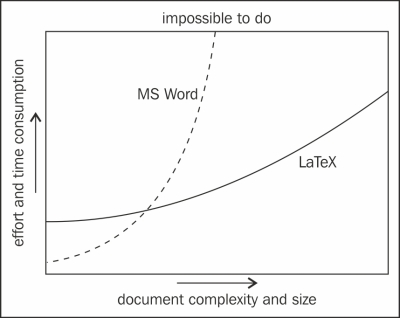
\includegraphics[width=0.5\linewidth]{Images/complexity_latex}
			\caption{Latex complexity}
			\label{fig:complexitylatex}
		\end{figure}
	\end{frame}
	\section{Result}
	\begin{frame}
		\frametitle{}
	\end{frame}
\end{document}